\documentclass{article}
\usepackage[utf8]{inputenc}
\usepackage{amsmath}
\usepackage{geometry}
\usepackage{multicol}
\usepackage{graphicx}
\usepackage{float}
\geometry{margin=1in}

\begin{document}

\newpage
\section*{Problema 1}









\textbf{Problema:}  
Se disolvieron 90 mL de alcohol etílico (\(C_2H_6O\), \(\rho_{C_2H_6O} = 0.789 \, \text{g/cm}^3\)) en 460 mL de agua (\(\rho_{H_2O} = 1 \, \text{g/mL}\)). Determinar:

\begin{itemize}
    \item[a)] Masa de soluto y solvente.
    \item[b)] Mol de soluto y solvente.
    \item[c)] Densidad de la solución.
\end{itemize}



% \begin{multicols}{2} % Divide el contenido en dos columnas.
\noindent\textbf{Datos:} % Define la sección de datos en la columna izquierda.
\begin{itemize}
    \item Masa molar (MM) de \(C_2H_6O = 46 \, \text{g/mol}\)
    \item Masa molar (MM) de \(H_2O = 18 \, \text{g/mol}\)
\end{itemize}
% \begin{figure}[H]
%     \begin{minipage}[t]{0.3\textwidth} % Define un espacio del 30% del ancho del texto.
%         \raggedright % Alinea a la izquierda dentro del minipage.
%         \includegraphics[width=\linewidth, height=2cm]{./problema10_diagrama.png} % Usa todo el ancho disponible en el minipage.
%         \caption{Diagrama del \\ problema}
%     \end{minipage}
% \end{figure}

\textbf{} % Define las variables y fórmulas utilizadas en el problema.
\begin{itemize}
\item V$_{\text{C}_2\text{H}_6\text{O}}$ = 40 mL (volumen de etanol)
\item V$_{\text{H}_2\text{O}}$ = 460 mL (volumen de agua)
\item $\rho_{\text{C}_2\text{H}_6\text{O}}$ = 0.789 g/mL (densidad del etanol)
\item $\rho_{\text{H}_2\text{O}}$ = 1 g/mL (densidad del agua)
\end{itemize}

% \columnbreak % Indica el cambio a la columna derecha.

\noindent\textbf{Resolución:} % Define la sección para los incisos y la resolución del problema.

\textbf{a) Masa de cada componente:}

\begin{align*}
    m_{\text{C}_2\text{H}_6\text{O}} &= 40 \, \text{mL} \times 0.789 \, \frac{\text{g}}{\text{mL}} = 31.56 \, \text{g} \\[10pt]
    m_{\text{H}_2\text{O}} &= 460 \, \text{mL} \times 1 \, \frac{\text{g}}{\text{mL}} = 460 \, \text{g} \\[10pt]
    m_{\text{solución}} &= 31.56 \, \text{g} + 460 \, \text{g} = 491.56 \, \text{g solución}
\end{align*}

\textbf{b) Moles de cada componente:}

\begin{align*}
    n_{\text{C}_2\text{H}_6\text{O}} &= \frac{31.56 \, \text{g}}{46 \, \frac{\text{g}}{\text{mol}}} = 0.686 \, \text{mol soluto} \\[10pt]
    n_{\text{H}_2\text{O}} &= \frac{460 \, \text{g}}{18 \, \frac{\text{g}}{\text{mol}}} = 25.556 \, \text{mol solvente} \\[10pt]
    n_{\text{solución}} &= 0.686 \, \text{mol} + 25.556 \, \text{mol} = 26.242 \, \text{mol solución}
\end{align*}

\textbf{c) Volumen total y densidad de la solución:}

\begin{align*}
    V_{\text{solución}} &= 40 \, \text{mL} + 460 \, \text{mL} = 500 \, \text{mL solución} \\[10pt]
    \rho_{\text{solución}} &= \frac{491.56 \, \text{g}}{500 \, \text{mL}} = 0.983 \, \frac{\text{g}}{\text{mL}}
\end{align*}

% \end{multicols} % Finaliza la división en dos columnas.









\newpage
\section*{Problema 2}
\textbf{Problema:}
Se mezclaron 75 g de NaCl en 460.71 g de H$_2$O, obteniéndose una solución salina con una densidad igual a 1.45. Determinar:

\begin{itemize} \item[a)] Masa de la solución y volumen de la solución. \item[b)] Mol de soluto, solvente y solución. \end{itemize}

\begin{itemize} \item Masa molar (MM) de NaCl = 58.5 g/mol \item Masa molar (MM) de H$_2$O = 18 g/mol \end{itemize}

% \begin{multicols}{2} % Divide el contenido en dos columnas.
\noindent\textbf{Datos:} % Define la sección de datos en la columna izquierda.

% \begin{figure}[H]
%     \begin{minipage}[t]{0.3\textwidth} % Define un espacio del 30% del ancho del texto.
%         \raggedright % Alinea a la izquierda dentro del minipage.
%         \includegraphics[width=\linewidth, height=2cm]{./problema11_diagrama.png} % Usa todo el ancho disponible en el minipage.
%         \caption{Diagrama del \\ problema}
%     \end{minipage}
% \end{figure}

\textbf{} % Define las variables y fórmulas utilizadas en el problema.
\begin{itemize}
\item m$_{\text{NaCl}}$ = 75 g (masa de cloruro de sodio)
\item m$_{\text{H}_2\text{O}}$ = 460.71 g (masa de agua)
\item $\rho_{\text{solución}}$ = 1.45 g/mL (densidad de la solución)
\end{itemize}

% \columnbreak % Indica el cambio a la columna derecha.

\noindent\textbf{Resolución:} % Define la sección para los incisos y la resolución del problema.

\textbf{a) Masa y volumen de la solución:}

\begin{align*}
    m_{\text{solución}} &= 75 \, \text{g} + 460.71 \, \text{g} = 535.71 \, \text{g solución} \\[10pt]
    V_{\text{solución}} &= \frac{535.71 \, \text{g solución}}{1.45 \, \frac{\text{g}}{\text{mL}}} = 369.46 \, \text{mL solución}
\end{align*}

\textbf{b) Moles de soluto y solvente:}

\begin{align*}
    n_{\text{NaCl}} &= \frac{75 \, \text{g}}{58.5 \, \frac{\text{g}}{\text{mol}}} = 1.28 \, \text{mol soluto} \\[10pt]
    n_{\text{H}_2\text{O}} &= \frac{460.71 \, \text{g}}{18 \, \frac{\text{g}}{\text{mol}}} = 25.60 \, \text{mol solvente} \\[10pt]
    n_{\text{solución}} &= 1.28 \, \text{mol} + 25.60 \, \text{mol} = 26.88 \, \text{mol solución}
\end{align*}

% \end{multicols} % Finaliza la división en dos columnas.









\newpage
\section*{Problema 3}
\textbf{Problema:}
Se disuelven 30 g de K$_2$Cr$_2$O$_7$ con un grado de pureza del 80\%. Determina la masa de solución de dicromato de potasio y la cantidad de moles de la solución.

Se emplearon 500 mL de agua.

\begin{itemize} \item Masa molar (MM) de K$_2$Cr$_2$O$_7$ = 294 g/mol \item Masa molar (MM) de H$_2$O = 18 g/mol \item Volumen de agua utilizado = 500 g H$_2$O \end{itemize}


% \begin{multicols}{2} % Divide el contenido en dos columnas.
\noindent\textbf{Datos:} % Define la sección de datos en la columna izquierda.

\begin{figure}[H]
    \begin{minipage}[t]{0.3\textwidth} % Define un espacio del 30% del ancho del texto.
        \raggedright % Alinea a la izquierda dentro del minipage.
        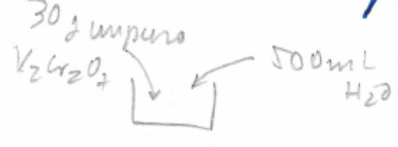
\includegraphics[width=\linewidth, height=2cm]{./problema3_diagrama.png} % Usa todo el ancho disponible en el minipage.
        \caption{Diagrama del \\ problema}
    \end{minipage}
\end{figure}

\textbf{} % Define las variables y fórmulas utilizadas en el problema.
\begin{itemize}
\item m$_{\text{K}_2\text{Cr}_2\text{O}_7, \text{impuro}}$ = 30 g (masa impura de dicromato de potasio)
\item V$_{\text{H}_2\text{O}}$ = 500 mL (volumen de agua)
\item Pureza de $\text{K}_2\text{Cr}_2\text{O}_7$ = 80\%
\item MM$_{\text{K}_2\text{Cr}_2\text{O}_7}$ = 294 g/mol (masa molar de dicromato de potasio)
\end{itemize}

% \columnbreak % Indica el cambio a la columna derecha.

\noindent\textbf{Resolución:} % Define la sección para los incisos y la resolución del problema.

\textbf{a) Masa de $\text{K}_2\text{Cr}_2\text{O}_7$ puro:}

\begin{align*}
    m_{\text{K}_2\text{Cr}_2\text{O}_7, \text{puro}} &= 30 \, \text{g impuro} \times \frac{80 \, \text{g puro}}{100 \, \text{g impuro}} = 24 \, \text{g} \, \text{K}_2\text{Cr}_2\text{O}_7
\end{align*}

\textbf{b) Masa total de la solución:}

\begin{align*}
    m_{\text{solución}} &= 24 \, \text{g} + 500 \, \text{g} = 524 \, \text{g solución}
\end{align*}

\textbf{c) Moles de soluto y solvente:}

\begin{align*}
    n_{\text{K}_2\text{Cr}_2\text{O}_7} &= \frac{24 \, \text{g}}{294 \, \frac{\text{g}}{\text{mol}}} = 0.082 \, \text{mol} \\[10pt]
    n_{\text{H}_2\text{O}} &= \frac{500 \, \text{g}}{18 \, \frac{\text{g}}{\text{mol}}} = 27.778 \, \text{mol} \\[10pt]
    n_{\text{solución}} &= 0.082 \, \text{mol} + 27.778 \, \text{mol} = 27.860 \, \text{mol solución}
\end{align*}

% \end{multicols} % Finaliza la división en dos columnas.









\newpage
\section*{Problema 4}
\textbf{Problema:}
Se necesitan mezclar 27 g (esto es lo que se debe disolver) de hidróxido de sodio (NaOH) con 15\% de impurezas con 830 g de agua. Determinar la masa de la solución de NaOH preparada y el volumen de la misma si se mide una densidad de 1.01, a la vez indicar los moles de soluto, solvente y solución.

% \begin{multicols}{2} % Divide el contenido en dos columnas.

\noindent\textbf{Datos:} % Define la sección de datos en la columna izquierda.

\begin{figure}[H]
    \begin{minipage}[t]{0.3\textwidth} % Define un espacio del 30% del ancho del texto.
        \raggedright % Alinea a la izquierda dentro del minipage.
        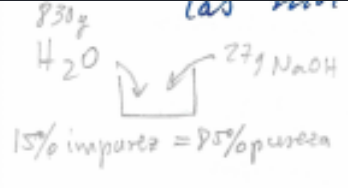
\includegraphics[width=\linewidth, height=2cm]{./problema4_diagrama.png} % Usa todo el ancho disponible en el minipage.
        \caption{Diagrama del \\ problema}
    \end{minipage}
\end{figure}

\begin{itemize}
\item m$_{\text{H}_2\text{O}}$ = 830 g (masa de agua)
\item V$_{\text{solución}}$ = 857.9 mL (volumen de la solución)
\item MM$_{\text{NaOH}}$ = 40 g/mol (masa molar de NaOH)
\item MM$_{\text{NaOH, impuro}}$ = 40 g/mol (masa molar de NaOH impuro)
\item $\rho_{\text{solución}}$ = 1.1 g/mL (densidad de la solución)
\item Porcentaje de pureza = 85\%
\end{itemize}

% \columnbreak % Indica el cambio a la columna derecha.

\noindent\textbf{Resolución:} % Define la sección para la resolución del problema.

\textbf{a) Masa total de la solución:}

\begin{align*}
    m_{\text{solución}} &= 27 \, \text{g} + 830 \, \text{g} = 857 \, \text{g solución}
\end{align*}

\textbf{b) Volumen de la solución basado en la densidad:}

\begin{align*}
    V_{\text{solución}} &= 857 \, \text{g solución} \times \frac{1 \, \text{mL solución}}{1.01 \, \text{g solución}} = 848.51 \, \text{mL solución}
\end{align*}

\textbf{c) Número de moles de NaOH:}

\begin{align*}
    n_{\text{NaOH}} &= 27 \, \text{g NaOH} \times \frac{1 \, \text{mol}}{40 \, \text{g}} = 0.675 \, \text{mol NaOH}
\end{align*}

\textbf{d) Número de moles de agua:}

\begin{align*}
    n_{\text{H}_2\text{O}} &= 830 \, \text{g H}_2\text{O} \times \frac{1 \, \text{mol}}{18 \, \text{g}} = 46.111 \, \text{mol H}_2\text{O}
\end{align*}

\textbf{e) Número total de moles en la solución acuosa de NaOH:}

\begin{align*}
    n_{\text{solución}} &= 0.675 \, \text{mol NaOH} + 46.111 \, \text{mol H}_2\text{O} = 46.786 \, \text{mol solución}
\end{align*}

\textbf{f) Masa de NaOH impuro necesaria para obtener la cantidad pura deseada:}

\begin{align*}
    m_{\text{NaOH, agregar}} &= 27 \, \text{g puro} \times \frac{1 \, \text{g impuro}}{0.85 \, \text{g puro}} = 31.76 \, \text{g impuro}
\end{align*}

% \end{multicols} % Finaliza la división en dos columnas.
\noindent\rule{\textwidth}{0.5pt}
\textbf{Pero si son 27g impuro(es decir agregado) entonces cambia todo a:}

\noindent\textbf{Resolución:} % Define la sección para la resolución del problema.

\textbf{a) Masa de NaOH puro:}

\begin{align*}
    m_{\text{NaOH, puro}} &= 27 \, \text{g impuro} \times \frac{85 \, \text{g puro}}{100 \, \text{g impuro}} = 22.95 \, \text{g NaOH puro}
\end{align*}

\textbf{b) Masa total de la solución:}

\begin{align*}
    m_{\text{solución}} &= 22.95 \, \text{g NaOH} + 830 \, \text{g H}_2\text{O} = 852.95 \, \text{g solución}
\end{align*}
\newpage
\textbf{c) Volumen de la solución basado en la densidad:}

\begin{align*}
    V_{\text{solución}} &= 852.95 \, \text{g solución} \times \frac{1 \, \text{mL solución}}{1.01 \, \text{g solución}} = 844.5 \, \text{mL solución}
\end{align*}

\textbf{d) Número de moles de NaOH:}

\begin{align*}
    n_{\text{NaOH}} &= \frac{22.95 \, \text{g NaOH}}{40 \, \frac{\text{g}}{\text{mol}}} = 0.57375 \, \text{mol NaOH} \, (\text{soluto})
\end{align*}

\textbf{e) Número de moles de agua:}

\begin{align*}
    n_{\text{H}_2\text{O}} &= \frac{830 \, \text{g H}_2\text{O}}{18 \, \frac{\text{g}}{\text{mol}}} = 46.11 \, \text{mol H}_2\text{O} \, (\text{solvente})
\end{align*}

\textbf{f) Número total de moles en la solución:}

\begin{align*}
    n_{\text{solución}} &= 0.57375 \, \text{mol NaOH} + 46.11 \, \text{mol H}_2\text{O} = 46.685 \, \text{mol de solución acuosa de NaOH}
\end{align*}










\newpage
\section*{Problema 5}
\textbf{Problema:}
Determina la masa de AlCl$_3$•10H$_2$O necesaria para disolver 60 g de soluto en 700 mL de agua. Calcula los moles de soluto, solvente y solución, y predice el volumen de la solución que se prepara.

% \begin{multicols}{2} % Divide el contenido en dos columnas.

\noindent\textbf{Datos:} % Define la sección de datos en la columna izquierda.

\begin{figure}[H]
    \begin{minipage}[t]{0.3\textwidth} % Define un espacio del 30% del ancho del texto.
        \raggedright % Alinea a la izquierda dentro del minipage.
        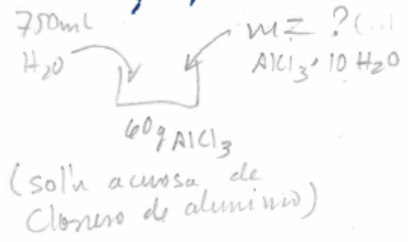
\includegraphics[width=\linewidth, height=2cm]{./problema5_diagrama.png} % Usa todo el ancho disponible en el minipage.
        \caption{Diagrama del \\ problema}
    \end{minipage}
\end{figure}

\begin{itemize}
\item V$_{\text{H}_2\text{O}}$ = 750 mL (volumen de agua)
\item m$_{\text{AlCl}_3}$ = 60 g (masa de cloruro de aluminio)
\item MM$_{\text{s.a.}}$ = 133.5 g/mol (masa molar de AlCl$_3$ anhidro)
\item MM$_{\text{s.h.}}$ = 313.5 g/mol (masa molar de AlCl$_3\cdot10\text{H}_2\text{O}$ hidratado)
\item $\rho_{\text{solución}}$ = 1 g/mL (densidad de la solución)
\end{itemize}

% \columnbreak % Indica el cambio a la columna derecha.

\noindent\textbf{Resolución:} % Define la sección para la resolución del problema.

\textbf{a) Masa de la sal hidratada:}

\begin{align*}
    m_{\text{sal hidratada}} &= 60 \, \text{g} \times \frac{313.5 \, \text{g sh}}{133.5 \, \text{g sa}} = 140.90 \, \text{g (AlCl}_3 \cdot 10\text{H}_2\text{O)}
\end{align*}

\textbf{b) Masa total de la solución:}

\begin{align*}
    m_{\text{solución}} &= 140.90 \, \text{g sal hidratada} + 750 \, \text{g H}_2\text{O} = 890.90 \, \text{g solución}
\end{align*}

\textbf{c) Masa del solvente (agua):}

\begin{align*}
    m_{\text{solvente}} &= 890.90 \, \text{g solución} - 60 \, \text{g AlCl}_3 = 830.90 \, \text{g solvente}
\end{align*}

\textbf{d) Número de moles de soluto:}

\begin{align*}
    n_{\text{soluto}} &= \frac{60 \, \text{g AlCl}_3}{133.5 \, \frac{\text{g}}{\text{mol}}} = 0.449 \, \text{mol soluto}
\end{align*}

\textbf{e) Número de moles de solvente:}

\begin{align*}
    n_{\text{solvente}} &= \frac{830.90 \, \text{g H}_2\text{O}}{18 \, \frac{\text{g}}{\text{mol}}} = 46.161 \, \text{mol solvente}
\end{align*}

\textbf{f) Número total de moles en la solución:}

\begin{align*}
    n_{\text{solución}} &= 0.449 \, \text{mol soluto} + 46.161 \, \text{mol solvente} = 46.610 \, \text{mol solución}
\end{align*}

\textbf{g) Volumen de la solución basado en la densidad:}

\begin{align*}
    V_{\text{solución}} &= 890.90 \, \text{g solución} \times \frac{1 \, \text{mL}}{1 \, \text{g}} = 890.90 \, \text{mL}
\end{align*}

% \end{multicols} % Finaliza la división en dos columnas.










\newpage
\section*{Problema 6}
\textbf{Problema:}
Se mezclan 150 g de Na$_2$C$_2$O$_4$•4H$_2$O con 1250 mL de H$_2$O. Determinar:

\begin{itemize} \item[a)] Masa de soluto, solvente y solución. \item[b)] Mol de soluto, solvente y solución. \item[c)] Densidad de la solución, si el volumen volumétrico alcanzó el aforo de 1500 mL. \end{itemize}

% \begin{multicols}{2} % Divide el contenido en dos columnas.

\noindent\textbf{Datos:} % Define la sección de datos en la columna izquierda.
\begin{figure}[H]
    \begin{minipage}[t]{0.3\textwidth} % Define un espacio del 30% del ancho del texto.
        \raggedright % Alinea a la izquierda dentro del minipage.
        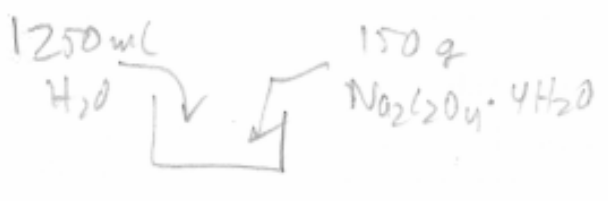
\includegraphics[width=\linewidth, height=2cm]{./problema6_diagrama.png} % Usa todo el ancho disponible en el minipage.
        \caption{Diagrama del \\ problema}
    \end{minipage}
\end{figure}
\begin{itemize}
\item V$_{\text{H}_2\text{O}}$ = 1250 mL (volumen de agua)
\item m$_{\text{Na}_2\text{C}_2\text{O}_4\cdot4\text{H}_2\text{O}}$ = 150 g (masa de oxalato de sodio hidratado)
\item MM$_{\text{Na}_2\text{C}_2\text{O}_4}$ = 134 g/mol (masa molar de Na$_2$C$_2$O$_4$ anhidro)
\item MM$_{\text{Na}_2\text{C}_2\text{O}_4\cdot4\text{H}_2\text{O}}$ = 206 g/mol (masa molar de Na$_2$C$_2$O$_4\cdot4\text{H}_2\text{O} $)
\end{itemize}

% \columnbreak % Indica el cambio a la columna derecha.

\noindent\textbf{Resolución:} % Define la sección para la resolución del problema.

\textbf{a) Masa del soluto (Na$_2$C$_2$O$_4$):}

\begin{align*}
    m_{\text{soluto}} &= 150 \, \text{g s.h.} \times \frac{134 \, \text{g sa}}{206 \, \text{g sh}} = 97.57 \, \text{g Na}_2\text{C}_2\text{O}_4
\end{align*}

\textbf{b) Masa total de la solución y del solvente (agua):}

\begin{align*}
    m_{\text{solución}} &= 150 \, \text{g s.h.} + 1250 \, \text{g H}_2\text{O} = 1400 \, \text{g solución} \\[10pt]
    m_{\text{solvente}} &= 1400 \, \text{g} - 97.57 \, \text{g} = 1302.43 \, \text{g H}_2\text{O}
\end{align*}

\textbf{c) Número de moles de soluto y solvente:}

\begin{align*}
    n_{\text{soluto}} &= \frac{97.57 \, \text{g}}{134 \, \frac{\text{g}}{\text{mol}}} = 0.728 \, \text{mol} \\[10pt]
    n_{\text{solvente}} &= \frac{1302.43 \, \text{g}}{18 \, \frac{\text{g}}{\text{mol}}} = 72.357 \, \text{mol}
\end{align*}

\textbf{d) Número total de moles en la solución:}

\begin{align*}
    n_{\text{solución}} &= 0.728 \, \text{mol soluto} + 72.357 \, \text{mol solvente} = 73.085 \, \text{mol solución}
\end{align*}

\textbf{e) Densidad de la solución:}

\begin{align*}
    \rho_{\text{solución}} &= \frac{1400 \, \text{g solución}}{1000 \, \text{mL solución}} = 0.933 \, \frac{\text{g}}{\text{mL}}
\end{align*}

% \end{multicols} % Finaliza la división en dos columnas.

\end{document}